\chapter{Discussion}\label{sec:discussion}

In this chapter, we discuss advantages and disadvantages of the different 
models developed in this thesis and competitor models, justifying contributions 
of this thesis.  In addition, we address possible criticisms and other 
tradeoffs and design choices that are of importance beyond raw accuracy.  
Performance of the different models in terms of part localization accuracy is 
in~\secref{system-results}.

\section{The case for image-dependent interactions}

At the time of publication, CPS was significantly better than all modern ``in 
the wild'' pose estimation approaches 
\citep{ferrari08,eichner09,devacrf,andriluka09}.  CPS was the only one to use 
image-dependent pairwise cues.  These other systems focused on either 
pre-processing to reduce the state space or improving unary potentials via 
foreground color estimation, and all performed inference relying ultimately on 
edge-based unary potentials and simple geometric displacement pairwise cues as 
in the classical PS model (\secref{ps}).


Recently, \citet{deva2011} introduced a multi-modal model of pose that competes 
with CPS. However, empirical results indicate that CPS generalizes better than 
\citet{deva2011}---both models applied to the Pascal dataset were trained on 
Buffy.  Furthermore, two years after its introduction in the literature, CPS is 
still the best performing model in the less precise regime 
(\figref{results-buffy-pascal}).  One of the reasons for the lack of precision 
is the coarser nature of our features: whereas \citet{deva2011} can evaluate 
placements to the granularity of a HoG cell, many of our features are more 
coarsely described and/or discretized---\eg, is the part guess near a contour, 
is the part guess in the foreground color.

In a more controlled setting, we see that a classical PS model coupled with 
just one image-dependent interaction feature---contour 
continuity---significantly improves performance (\figref{ablative}).

The benefits of image-dependent interactions is further reinforced by the 
performance by our video pose estimation model.  The Ensemble of Stretchable 
Models exploits a variety of across-body and across-frame image interactions 
and significantly outperfoms methods with fewer interactions.

In general, our cascade approach is a principled framework that frees us from 
restricting our models to simplified pairwise potentials of the form 
$\phi_{ij}(y_i - y_j)$. This allows much more flexibility in the future 
incorporating more pairwise and even higher-order features. 

\section{More features or more modes?}
As first mentioned in~\secref{llps}, there are two major approaches for 
improving pose accuracy in recent years: adding more features, \eg CPS, ESM and 
\citet{ferrari08,eichner09,ddtran}, or adding more modes, \eg LLPS and 
\citet{dpm,wang2011,deva2011,johnson11}.  

Currently, LLPS slightly underperforms CPS and~\citet{deva2011}.  However, it 
ambitiously uses an order of magnitude more modes than existing multi-modal 
approaches.  It may be suffering due the computational difficulties preventing 
joint training of different modes, and lack of a sufficiently sized dataset.  
\figref{llps-learning-curve} indicates further improvement with larger 
datasets.

\begin{figure}[htb!]
\centering
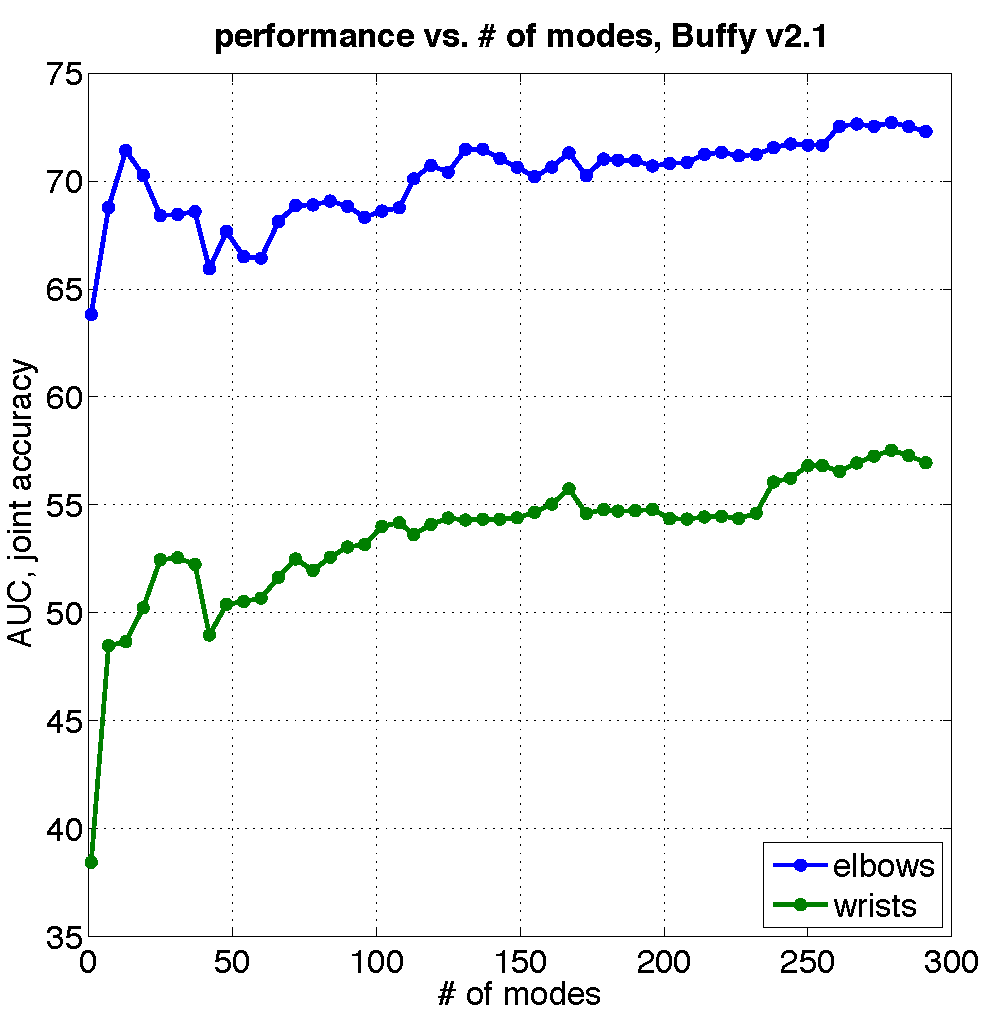
\includegraphics[width=0.59\linewidth]{figs/llps-learning-curve.pdf}
\caption[Test accuracy versus number of local neighborhood modes in LLPS.]{
\label{fig:llps-learning-curve} We show test set accuracy on Buffy for LLPS, 
measured by area under the joint precision curve.  For this analysis, we added 
modes to our model in the order they were chosen by our greedy mode selection 
process / basis pursuit (\secref{calib}).  We stopped at the point 
cross-validation determined there were no more beneficial modes to add. The 
increasing performance as a function of number of modes implies that having a 
larger training set with more local neighborhoods would further improve 
accuracy of our system.  It is important to note that training and inference 
scale linearly (and are parallelizable) with the number of modes in our method, 
so we intend to investigate this for future work.}
\end{figure}


Ultimately, these research directions are complementary, and an ideal model 
would use a combination of rich features and multiple modes. Additional feature 
types (\eg, segments, contours, optical flow, depth) incurs an additional cost 
to obtain, but adds to the generalization capabilities of the model. Additional 
modes allows for more specific modeling of different scenarios, but requires 
more training data to estimate parameters accurately.  This leaves a large 
space of possible models combining the two approaches.

\section{Joints or limbs?}

The ESM model introduced a joint-based 2D representation of pose.  At the same 
time, \citet{deva2011} also introduced a model based on joints and limb 
midpoints as basic units of inference.  This approach has clear benefits for 
easily capturing foreshortening and scale.  It has the seeming disadvantage of 
not being able to capture limb-pair features with a pairwise model.  However, 
this is not a fundamental limitation.  Especially using cascaded inference 
techniques we should not shy away from describing higher order cliques in the 
future.  In general, the scope of the basic atomic unit for inference (the 
inference variables) need not be dictated by the scope of the largest clique we 
capture in our model.  Joint-based models are worth exploring further.  In 
particular, we expect an Ensemble of Stretchable Models approach applied to 
{\em single frame} pose estimation to work well.

\section{Detection, localization, or both?}

Some pose estimation models use as a selling point that they work well for both 
person detection---finding where a person in at different scales in an image 
{\em and} pose estimation---localizing there body parts.  In particular 
\citet{andriluka09} and \citet{deva2011} do this.  The benefits of these 
approaches are that they are easy to use: one function to both find a person 
and find their body parts.  Our approach on the other hand, is really two step 
when given an image: (1) detect the person with a dedicated person detector, 
and (2) run our pose models on the detected person.  This is a slightly more 
cumbersome procedure. 

We believe that detection and localization are fundamentally different tasks 
and should be decoupled.  In detection, we wish to generalize over all poses 
and determine how to discriminate any pose from background clutter---a 
detection is correct even when a pose is incorrect, and a detector must also 
have some notion of global confidence to determine, over all possible image 
patches, whether it is a person or not.  A pose estimator works under the 
assumption that a pose is present, and is correct only if it predicts the right 
pose versus combinatorially many wrong poses.

One model that attempts to perform both tasks is bound to perform only as well 
as it could tuned to each task independently, and probably worse.  It may be 
that PS models are the right family of models for both detection and 
localization---they have attractive benefits for generalizing over poses with 
deformations and obstructions in addition to localizing pose---and they should 
be used for both.  However, a detection model should be trained with the task 
of detection in mind, and a pose estimation model should be trained for pose 
estimation. 

\section{Everything and the kitchen sink: a bug or a feature?}
Some of the main contributions of this thesis are technical innovations that 
allow us to include a smorgasbord of features.  The goal was to include as many 
feature modalities as possible in our CPS and ESM models.  Having so many 
features makes it difficult to determine exactly what is contributing to the 
success of our model.  

From a machine learning standpoint, this is an attractive aspect of our system: 
given training data, we can try everything and see what works.  From a computer 
vision standpoint, this is a disadvantage---it is difficult to gain insight 
into why the model is performing well exactly.

We take a functional, application-driven approach towards computer vision, and 
consider our problem on pose estimation as engineering rather than perceptual 
science.  The inability to measure the individual performance of components in 
any complex system is inevitable---the whole is greater than the sum of its 
parts.  We provide individual feature analysis in~\figref{ablative}, and make 
convincing arguments that the features and interactions we include are 
beneficial.  We make no statement as to which features are the ``best'', in any 
sense other than their contribution to final system performance.

\section{Accuracy, speed, simplicity}

When developing our CPS and ESM models, we focused our attention and obtaining 
the best performing, computationally tractable system.  Besides raw 
performance, practitioners care as much about {\em speed}---does the system run 
quickly?---and {\em simplicity}---how long does it take for me to download, 
compile, understand, run and/or re-implement in a language of choice?  One of 
the motivations of LLPS and attractiveness of~\citet{deva2011} is their speed 
and simplicity, in terms of image features (only HoG) and lines of code.

To wit, while performing only slight better than LPPS, CPS and ESM have a 
significant feature overhead, involving Normalized Cuts segmentation and gPb 
and in total, hundreds of different feature types.  These two approaches take 5 
to 10 minutes per image.  Further, the work of~\citet{eichner09} involves 
iterative re-estimation of part color models, iterative inference with 
different trees, and graphcut.  Their public implementation takes 10.5 seconds 
per image.

LLPS, on the same machine, takes 11.0 seconds per image using 1 core.  However, 
since LLPS inference is trivially parallelizable at the level of local models, 
using 8 cores reduces this time in practice to 4.1 seconds on average, 1.5 
seconds of which are spent running the un-optimized hand detector feature.  We 
expect further linear speedup with more cores.


\citet{deva2011}'s model takes 1.6 seconds to run on our machines, using 32 
features of signed and unsigned edge and color histograms.  Their model uses 
just a few modes per part, but their inference is quadratic in the number of 
modes, making it unclear how they might scale to hundreds of modes like our 
method uses, although they note in their paper more modes leads to better 
performance.

We believe that, moving forward, models with any combination of the three 
objects {\em accuracy, speed, simplicity} are all worthwhile, even independent 
of the others.  Any current system's slowness today will likely be a non-issue 
in 5-10 years with the advent of faster CPUs. Anecdotally, at time of 
publication two years ago, the CPS system took 5 minutes and 15 seconds on an 
Intel Xeon E5450 CPU @ 3.00GHz with 8 cores.  Today, at roughly the same price 
and consumer availability, the system runs in 3 minutes on an AMD Opteron 4284 
CPU @ 3.00 GHz with 16 cores.

\chapter{Future directions}

what will it take to work?
  + more data
  + more computation

does the right cost function exist?

\chapter{Conclusion}

This thesis proposes advancements in 2D human pose estimation models to improve 
upon state-of-the-art performance.  Specifically, previously proposed pictorial 
structures models are handicapped by the needs of efficient inference tricks; 
forced to express simple pairwise cues that are only a function of parts' 
spatial relationships.  Further, the spatial relationship structure had to form 
a tree graph.

We push past the inference barrier in several ways, allowing us to include 
richer image-dependent interactions.  First, we proposed Cascaded Pictorial 
Structures ({\bf CPS}), a sequence of structured models that efficiently prune 
the state space of possible poses down to a manageable number.  This allows us 
to perform efficient exact inference without restrictions.  We exploit this by 
incorporating a variety of rich features from complementary sources, improving 
upon state-of-the-art PS approaches in single frame pose estimation.

We then extend this approach to handle pose estimation in video.  Maintaining a 
rich set of variable interactions in video creates a cyclic network of variable 
interactions, which is known to require inference inference exponential in the 
number of frames of video.  We maintain tractability through the use of a 
cascade step as in CPS, and an approximate inference method which decomposes 
the cyclic structure of interactions into an ensemble of tree graphs, which 
capture all the interactions of the cyclic network, with redundancies.  With 
this Ensemble of Stretchable Models ({\bf ESM}), approximate inference is only 
linear in the number of frames of video.  Furthermore, to handle fine-grained 
articulation and foreshortening effects often present in real video clips, we 
use a joint-based representation of pose, as opposed to a limb-based 
representation, hence our model is ``stretchable''.

Finally, we explore a complementary approach to the line of research that 
motivated CPS and ESM.  These methods focused on novel computational techniques 
that allowed us to add more and more features and rich interactions into our 
pose models, in the hope that more features would lead to better 
generalizability and performance accuracy.  Alternatively, in Local Linear 
Pictorial Structures ({\bf LLPS}), we focus instead explicitly on the 
non-linear, multi-modal nature of the problem, {\em not} by introducing more 
and more features, but instead modeling each local neighborhood with it's own 
PS model.  Local neighborhoods are defined as a function of closeness in 
appearance and pose centered at every training example, allowing us to 
preciesely model different modes of the input that result from different 
clothing, body types, and pose.

We show empirically that our models are state-of-the-art on competitive public 
datasets, verifying the worthiness of our modeling innovations: (1) cascades of 
structured models (2) ensemble of tree models (3) joint-based representations 
(4) local linear modeling.  All of these ideas are valuable contributions to 
the field of pose estimation, with potential to help in other domains involving 
structured problems as well.

Human pose estimation in the wild in its most general setting is still far from 
a solved problem, although we have made significant advances through the course 
of this research.  Moving forward, we expect further advances to be made with 
larger datasets, the computation capabilities to scale current approaches to an 
order of magnitude more data, and reconciling estimates of pose within the 
larger context of scene understanding.

Future improvements in pose accuracy seem promising and the dream of 
understanding human pose for a variety of applications is increasingly 
compelling given the advancements in robotics and the pervasiveness of cameras 
in our lives.  In conclusion, the future of pose estimation is bright.
